% -*- root: ../mainThesis.tex -*-
%
%
%  ▄█     █▄     ▄████████  ▄█        ▄█             ▄█  ███▄▄▄▄   ████████▄     ▄████████ ▀████    ▐████▀ 
% ███     ███   ███    ███ ███       ███            ███  ███▀▀▀██▄ ███   ▀███   ███    ███   ███▌   ████▀  
% ███     ███   ███    █▀  ███       ███            ███▌ ███   ███ ███    ███   ███    █▀     ███  ▐███    
% ███     ███  ▄███▄▄▄     ███       ███            ███▌ ███   ███ ███    ███  ▄███▄▄▄        ▀███▄███▀    
% ███     ███ ▀▀███▀▀▀     ███       ███            ███▌ ███   ███ ███    ███ ▀▀███▀▀▀        ████▀██▄     
% ███     ███   ███    █▄  ███       ███            ███  ███   ███ ███    ███   ███    █▄    ▐███  ▀███    
% ███ ▄█▄ ███   ███    ███ ███▌    ▄ ███▌    ▄      ███  ███   ███ ███   ▄███   ███    ███  ▄███     ███▄  
%  ▀███▀███▀    ██████████ █████▄▄██ █████▄▄██      █▀    ▀█   █▀  ████████▀    ██████████ ████       ███▄ 
%
\chapter{Well index calculation}
%
The well index is an essential part of well
placement optimization.
%
In a reservoir simulation, the flowing bottom hole pressure differs 
from the measured well block pressure. In order to connect the
two D. Peaceman introduced the
well index, or well transmisibillity factor, and
suggested a way to calculate it. We refer to Peaceman's
paper\cite{Peaceman_Paper} for a more in-depth explanation on 
the topic.
%
The bottom hole pressure determines the rate of flow
through the well, which again determines the production
rate of the well. So because the well index determines
the production rate, the objective function $J$ greatly
depends on it. This means that, if we wish to develop a good 
algorithm for the well placement problem optimization, 
it is essential to be able to calculate the well index
for all well blocks.
%
Peaceman's original paper only considered horizontal
wells, but new algorithms for slanted (i.e., not fully
horizontal) wells have been developed, three of which
are described by Shu in his report \cite{Shu_Paper}.
%
\section{Projection well index}
% 
In this thesis we will use the projection well index, 
originally developed by Jonathan Holmes \cite{Holmes},
which is described by Shu in Chapter 2 of his report.
%
The main assumptions of the model is a uniform Cartesian 
grid with single-phase radial flow without interaction 
with boundaries or other wells. In the projection well
index method, the well trajectory is projected onto three
orthogonal axes as shown in Figure \ref{fig:well_index}.
%
\begin{figure}[H]
	\centering
	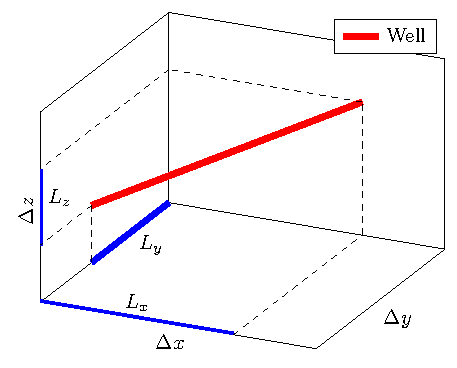
\includegraphics[width=0.80\textwidth]{figures/well_index/well_index.pdf}
	\caption{Well trajectory in a single well block projected 
			 onto the three axes. The projections have lengths $L_x$, $L_y$
			 and $L_z$, and the well block has dimensions $\Delta_x$, $\Delta_y$
			 and $\Delta_z$. This figure is a copy of the one used by Shu in
			 his report \cite{Shu_Paper}}
	\label{fig:well_index}
\end{figure}
%
The well index can now be calculated for slanted wells and
non-square blocks by first calculating the well index for
each direction with
%
\begin{align}
WI_x = \frac{2 \pi \sqrt{k_y k_z} L_x}{\ln \frac{r_{0,x}}{r_w} + s}, \quad WI_y = \frac{2 \pi \sqrt{k_x k_z} L_y}{\ln \frac{r_{0,y}}{r_w} + s}
\quad \text{and} \quad WI_z = \frac{2 \pi \sqrt{k_x k_y} L_z}{\ln \frac{r_{0,z}}{r_w} + s}, 
\end{align}
%
where $k_i$ is the permeability in direction $i$, $r_w$ is the 
wellbore radius, $s$ is the skin factor and
%
\begin{align}
r_{0,x} = 0.28 \frac{ \bigg( \Delta z^2 \left( \frac{k_y}{k_z} \right)^{\frac{1}{2}} +  \Delta y^2 \left( \frac{k_z}{k_y} \right)^{\frac{1}{2}} \bigg)^{\frac{1}{2}} }{ \left( \frac{k_y}{k_z} \right)^{\frac{1}{4}} + \left( \frac{k_z}{k_y} \right)^{\frac{1}{4}} }.
\end{align}
%
The functions $r_{0,y}$ and $r_{0,y}$ are defined in the 
same manner but with the indices $x, y$ and $z$ shifted.
%
At last we take the square root of the sum of the squares
of the directional well indices to get the well index for
the block
%
\begin{align}
WI = \sqrt{WI_x^2 + WI_y^2 + WI_z^2}.
\label{eq:well_index}
\end{align}
%
For the rest of 
this thesis we will simplify the equation by setting $s = 0$, 
i.e., neglecting the skin factor.
%
\section{Computing well trajectory and projection}
% 
In order to compute the well index with \eqref{eq:well_index}
we need not only determine which blocks are penetrated 
by the wells, but also determine the point of entry and
exit. This is done by first using a function called 
\texttt{GetblockEnvelopingPoint()}. This function simply iterates
over all the well blocks of the reservoir and returns the first
block that contains a given point. This is done by checking that
the point is on the correct side (i.e., towards the center of the 
well block) of every face of the block. Using this function on the 
start point will give us the well block that contains the 
starting point as shown in Figure \ref{fig:intersect_block_epsilon}.
%
\begin{figure}[H]
	\centering
	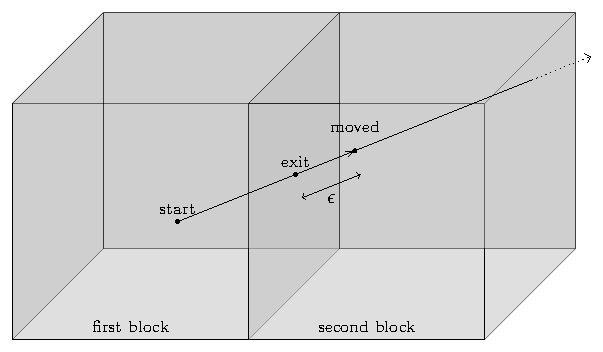
\includegraphics[width=0.80\textwidth]{figures/intersecting_wells/move_point_eps.pdf}
	\caption{Moving a small distance $\epsilon$ along the line segment
			 towards the end of the line segment will ensure that
			 we are completely inside the next block. In the new
			 block we can perform the same steps as we did in the previous block.}
	\label{fig:intersect_block_epsilon}
\end{figure}
%
We then find the intersection point between the well and 
this first block, which we will call the exit point of the well.
Now we have acquired the intersection points for the first well 
block. After this we simply move a sufficiently small 
distance $\epsilon$ from this exit point towards the end of 
the well, and call this new point moved point. With sufficiently
small we mean a small fraction ($\sim \frac{1}{100}$) of the shortest
well side length. Note that this could lead to numerical errors as
we might jump over some blocks if the intersection between the 
well and the block is very short. But if the length of the
intersection is very short, then value of the corresponding well 
index will be very small as well, thus we can neglect it. 
%
Now we can use
the same method as we did for the starting point to get the
intersection points of the second block, and this process can
be repeated until we reach the end of the well.
%
%
Because the corner coordinates of the well block are known, we can compute
the lengths $\Delta_x$, $\Delta_y$ and $\Delta_z$ for each side of the block.
Then we can find the unit vector $\textbf{u}_i$ for the direction of the sides
of the well block. Thus given a well block and its two intersection points,
$\textbf{p}_1$ and $\textbf{p}_2$, the projected well lengths $L_x$, $L_y$ 
and $L_z$ are given by 
%
\begin{align}
L_i = \big\langle (\textbf{p}_2 - \textbf{p}_1), \textbf{u}_i \big\rangle.
\end{align}
%
Supplying the permeabilities $k_i$ and wellbore radius $r_w$ and in the absence
of skin ($s = 0$), we can compute the well index of the block with \eqref{eq:well_index}.
%